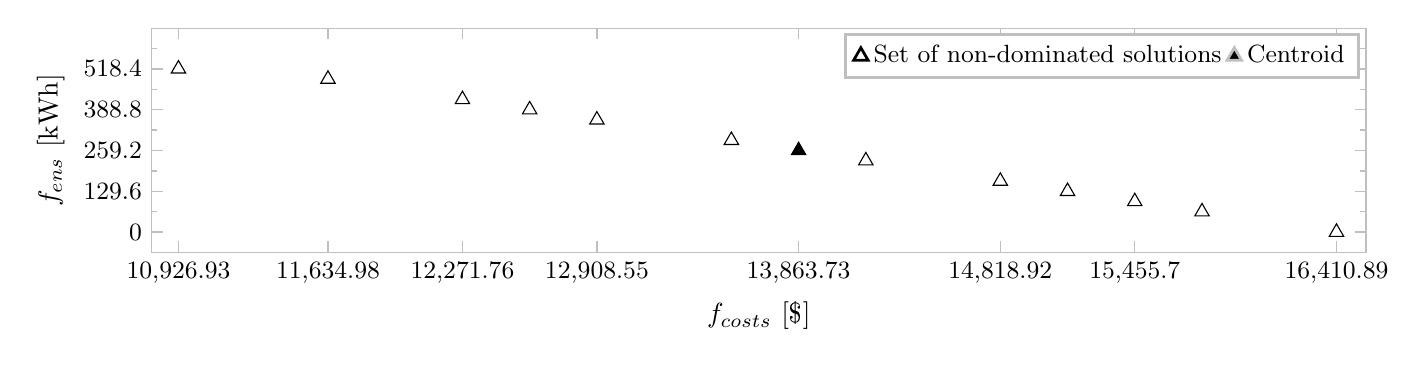
\begin{tikzpicture}
    \begin{axis}[
        %width=240pt,
        % height = 140pt,
        % x dir = reverse,
        y post scale = 0.5,
        x post scale = 2.25,
        xlabel={$f_{costs}$ [\$]},
        xlabel near ticks,
        % axis x line = bottom,
        % axis line shift = 10pt,
        ylabel={$f_{ens}$ [kWh]},
        ylabel near ticks,
        % axis y line = left,
        % axis line style={|-stealth},
        % axis x discontinuity=crunch,
        tick style = {line width = 0.5, color = lightgray, 
            major tick length=4pt,minor tick length=2pt, 
            minor y tick num =1, xtick = {10926.93, 11634.98, 12271.76,
            12908.55, 13863.73, 14818.92, 15455.70, 16410.89}
            },
        tick label style = {font=\small, ytick distance=129.6
            },
        xtick align = {inside},
        ytick align = {inside},
        % extra x ticks={10926.93},
        %extra x tick labels={10926.93},
        % label style = {font=\small},
        % legend style = {font=\footnotesize, at={(0.5,1.05)},    
        %     anchor=south, legend cell align=left, line width=0.5pt, 
        %     draw=lightgray, legend columns = 2}
        legend style = {font=\small, at={(0.995,0.98)},    
            anchor= north east, legend cell align=center, line width=1pt, 
            draw = lightgray, legend columns = 2},
        ymax=647,
        xmin=10800, xmax=16550,
        % enlarge x limits=0.05,
        axis line style = {line width = 0.5pt, lightgray},
        scaled ticks=false
        ]
    % % Best compromise point
    % \addplot[mark = triangle*, only marks, 
    %         mark size = 2.5pt] 
    % coordinates {
    % (10926.93,518.4)};
    % \addlegendentry{Best compromise point}

    % % Best Compromise utopia distance
    % \addplot[black, line width=1pt] 
    %     coordinates {
    %     (10926.93, 0)
    %     (10926.93, 518.4)
    %     };
    % \addlegendentry{Best compromise distance}
    
     % Set of non-dominated solutions 
    \addplot[mark = triangle, only marks, mark size = 3pt,
    black] 
    coordinates {
        (10926.93, 518.4)
        (11634.98, 486.0)
        % (11953.37, 453.6)
        (12271.76, 421.2)
        (12590.16, 388.8)
        (12908.55, 356.4)
        % (13226.95, 324.0)
        (13545.34, 291.6)
        % (13863.73, 259.2)
        (14182.13, 226.8)
        % (14110.87, 194.4)
        (14818.92, 162.0)
        (15137.31, 129.6)
        (15455.70, 97.2)
        % (15702.84, 32.4)
        (15774.10, 64.8)
        (16410.89, 0)               
        };
    \addlegendentry{Set of non-dominated solutions}
    
    % Compromise-utopia distances

    % \addplot[lightgray, dotted, line width=1pt] 
    %     coordinates {
    %     (10926.93, 0)
    %     (11634.98, 486.0)
    %     };
    % \addplot[lightgray, dotted, line width=1pt] 
    %     coordinates {
    %     (10926.93, 0)
    %     (11953.37, 453.6)
    %     };
    % \addplot[lightgray, dotted, line width=1pt] 
    %     coordinates {
    %     (10926.93, 0)
    %     (12271.76, 421.2)
    %     };
    % \addplot[lightgray, dotted, line width=1pt] 
    %     coordinates {
    %     (10926.93, 0)
    %     (12590.16, 388.8)
    %     };
    % \addplot[lightgray, dotted, line width=1pt] 
    %     coordinates {
    %     (10926.93, 0)
    %     (12908.55, 356.4)
    %     };
    % \addplot[lightgray, dotted, line width=1pt] 
    %     coordinates {
    %     (10926.93, 0)
    %     (13226.95, 324.0)
    %     };
    % \addplot[lightgray, dotted, line width=1pt] 
    %     coordinates {
    %     (10926.93, 0)
    %     (13545.34, 291.6)
    %     };
    % \addplot[lightgray, dotted, line width=1pt] 
    %     coordinates {
    %     (10926.93, 0)
    %     (13863.73, 259.2)
    %     };
    % \addplot[lightgray, dotted, line width=1pt] 
    %     coordinates {
    %     (10926.93, 0)
    %     (14182.13, 226.8)
    %     };
    % \addplot[lightgray, dotted, line width=1pt] 
    %     coordinates {
    %     (10926.93, 0)
    %     (14110.87, 194.4)
    %     };
    % \addplot[lightgray, dotted, line width=1pt] 
    %     coordinates {
    %     (10926.93, 0)
    %     (14818.92, 162.0)
    %     };
    % \addplot[lightgray, dotted, line width=1pt] 
    %     coordinates {
    %     (10926.93, 0)
    %     (15137.31, 129.6)
    %     };
    % \addplot[lightgray, dotted, line width=1pt] 
    %     coordinates {
    %     (10926.93, 0)
    %     (15455.70, 97.2)
    %     };
    % \addplot[lightgray, dotted, line width=1pt] 
    %     coordinates {
    %     (10926.93, 0)
    %     (15702.84, 32.4)
    %     };
    % \addplot[lightgray, dotted, line width=1pt] 
    %     coordinates {
    %     (10926.93, 0)
    %     (15774.10, 64.8)
    %     };
    % \addplot[lightgray, dotted, line width=1pt] 
    %     coordinates {
    %     (10926.93, 0)
    %     (16410.89, 0) 
    %     };
    % \addlegendentry{Compromise distances}

    % %Utopia point
    % \addplot [mark size = 2.5pt, black, only marks]
    %     coordinates {
    %     (10926.93, 0)
    %     };
    % Centroid
    \addplot [mark size = 3pt, only marks, mark = triangle*]
        coordinates {
        (13863.73, 259.2)
        };
    \addlegendentry{Centroid}
    % \node [coordinate, pin=above right:{Centroid}] at
    %     (axis cs: 13863.73, 259.2 ) {};
    % \node [coordinate, pin=above right:{Ideal Point}] at
    %     (axis cs: 10926.93, 0) {};
    \end{axis}
\end{tikzpicture}